\documentclass[a4paper,10pt,twocolumn,dvipdfmx]{jsarticle}
\usepackage[dvipdfmx]{graphicx}
\usepackage{tikz}
\usepackage{here}
\usepackage{array,booktabs}
\usetikzlibrary{patterns}

\newcommand{\Dt}{\Delta t}
\newcommand{\II}{I\hspace{-.1em}I}

\title{画像処理による粉粒体高速流動の画像情報の統計的処理}
%Comparative evaluation of autocorrelation function of time-dependent configuration of particulate/powdery systems in fast translational motion and the velocity of the apparent motion of them
\author{吉渡 匠汰}
\date{ } %change

%\setlength{\textwidth}{155truemm}
%\setlength{\fullwidth}{\textwidth}
%\setlength{\oddsidemargin}{37truemm}
%\addtolength{\oddsidemargin}{-1truein}
%\setlength{\topmargin}{30truemm}
%\setlength{\textheight}{237truemm}
%\addtolength{\topmargin}{-1truein}

\begin{document}
\twocolumn[
\maketitle
\begin{abstract}
直観的な視覚情報において「ふうあい」は重要な要素の一つである。しかし、そのふうあいを言語で説明することは難しく、「暗黙知の領域」とされてきた。だが、近年では0.1 msレベルでの撮影を手軽に行えるようになり、この領域の基礎研究が進められてきた。以前までの研究では粉や水のハイスピード映像を撮影し、目視によってその特徴を調査してきた。本研究では二値化画像処理を中心としたコンピュータによる解析を行うことで粉粒体落下運動の映像の自己相関関数$G(\Delta t)$を求めた。テクスチャ状の特徴と比較し、粉粒体の落下運動の映像を数値で説明することを試みた。 \par
\end{abstract}
] 

\section{物体の運動評価法}
物体の視覚情報を数値化する方法として、視覚情報の自己相関関数を計算する方法を考えた。自己相関関数とは1つのムービーについて、ある瞬間の映像が時間シフトした映像とどれだけ一致しているかという尺度である。自己相関関数を様々な粉粒体の落下映像について求めることとで、映像の変動を解析した。
\subsection{画像処理について}
物体の動きを正確に追うため本研究では二値化画像処理を用いている。二値化とは各画素について一定の閾値以下ならば白、そうでないならば黒にするという処理を施し、二色の画像を作成する処理である。運動する対象の色とギャップの大きい色を背景にして撮影し、二値化処理によって対象を白または黒で抜き出すことができる。 \par
二値化処理を施した画像の例として図\ref{fig:threshold}を示す。
\begin{figure}[H]
	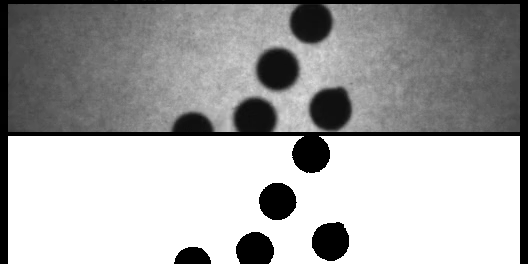
\includegraphics[clip,width=7.0cm]{bb_image.png}
	\caption{二値化画像の例 上:撮影された映像の1フレーム、下:二値化画像}
	\label{fig:threshold}
\end{figure}
\subsection{相関関数の評価方法}
まず画像間の類似性というものを考える。ここで類似性とは同一時系列上にある2つの画像がどれだけ似ているかという意味で用いているが、まずは類似性の数値化を試みた。そのためには類似性の具体的な定義を行う必要がある。本研究では次のように定義した、「画像間で色が一致しているピクセルの数[px]」。イメージ画像を図\ref{fig:exfall}に示す。比較する際にまずベースフレーム($t_0$時点)を一つ決める。次に$t_0+\Delta t$後の画像と比較する。色が一致するピクセル数を$S(\Delta t)$と表すことにする。$S(0)$は同じ画像同士の比較なので完全に一致するため、$S(0)$は比較画像のピクセル数に等しい。$\Delta t$が少しずれて、例えば$S(\frac{1}{5000})$のようになると$S(0)$よりも少し小さくなる。これを$0 \leq \Delta t \leq 0.1 [s]$の範囲で計算する。なお落下運動は定常なものであるため、$t_0$を適当に20点選び平均をとっている。 \par
$S(0 \leq \Delta t \leq 0.1)をS(0)$の値で割り、規格化した値を自己相関関数$G(\Delta t)$とする。$S(\Delta t)の範囲が0 \leq S(\Delta t) \leq S(0)であるから、相関関数G(\Delta t)の値域は0 \leq G(\Delta t) \leq 1となる$。
\begin{figure}[hbtp]
	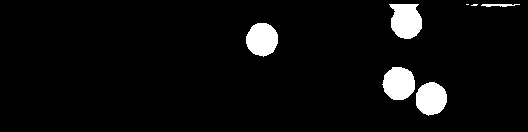
\includegraphics[clip,width=7.0cm]{0.png}
	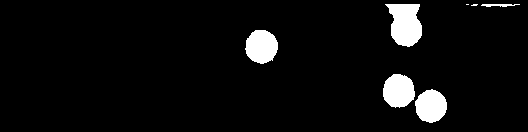
\includegraphics[clip,width=7.0cm]{3.png}
	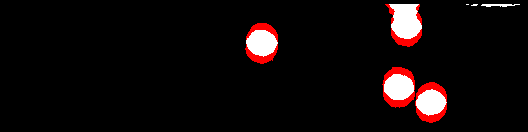
\includegraphics[clip,width=7.0cm]{0and3.png}
	\caption{画像比較のイメージ(上:t=0s,中央:$\frac{3}{5000}s$,下:比較) \newline $黒、白 \cdots 色が一致 ,赤 \cdots 色が不一致$}
	\label{fig:exfall}
\end{figure}
\subsection{相関関数の評価方法}

\section{測定方法}
測定に用いるのは落下装置とハイスピードカメラである。落下装置はダンボール箱を加工したもので、光を通したり撮影したりするための穴や物体を充填する漏斗とストッパーで構成されている。装置とカメラの位置関係を図\ref{fig:equip}に示す。2つの距離は70 cmとし、カメラに映っている範囲で物体の落下速度は約2 m/sとなるようにしている。
\subsection{物体の種類}
本研究で測定した物体は表\ref{tb:ballkind}に示す7種類である。 \\
\begin{table}[H]
	\caption{実験に使用した物体 \label{tb:ballkind}}
	\begin{tabular}{lr}
		\toprule
		種類 & 直径[mm] \\
		\midrule
		金属球 & 6.2 \\
		BB弾 & 6.0 \\
		発泡ポリスチレン & 1.54 \\
		砂(15〜20メッシュ) & 1 \\
		砂(20〜30メッシュ) & 0.7 \\
		海砂(150〜200メッシュ) & 0.08 \\
		ガラスビーズ & 0.02-0.08 \\
		水(白絵の具で着色) & - \\
		\bottomrule
	\end{tabular}
\end{table}

表\ref{tb:ballkind}で金属球、BB弾、発泡ポリスチレンは実際に測定したものだが、砂と海砂については表記されたメッシュ値を参考におおよその直径を決めている。 \par
カメラのシャッタースピードは5000 fps($\frac{1}{5000}秒に1回$)、露光時間は$\frac{1}{80000}秒$である。 \par
本研究においてほとんどの物体は黒背景にして白色で抜き出している。これは物体にライトを当てることによって物体が白っぽく映るためであるが、金属球については反射によって色のむらができてしまうため、白背景にして後ろから光を当てることにより黒で抜き出している。

\section{各物体の評価}
\subsection{相関関数}
実験で得られた各物体の相関関数を下記にまとめる。なお、グラフ中の略称については表\ref{tb:ballname}を参照のこと。図\ref{fig:overall}に0.1秒間の自己相関関数の変化を示す。砂や水といった物質は比較的相関が減少していないことがわかる。これらの物体は人の目から見ても帯状に連なって落ちていることがわかる。すなわち、粒ひとつひとつが独立して動くことがなく、なだらかな動きを見せるのである。このような場合撮影したどのフレームを見ても形は大きく変わっていない。 \par
\begin{table}[H]
	\caption{粉粒体の略称 \label{tb:ballname}}
	\begin{tabular}{lr}
		\toprule
		種類 & 略称 \\
		\midrule
		金属球 & Metal \\
		BB弾 & BB \\
		発泡ポリスチレン & EPS \\
		砂(15〜20メッシュ) & sand1520 \\
		砂(20〜30メッシュ) & sand2030 \\
		海砂(150〜200メッシュ) & seasand \\
		ガラスビーズ & glass \\
		水(白絵の具で着色) & water \\
		\bottomrule
	\end{tabular}
\end{table}
\begin{figure}[H]
	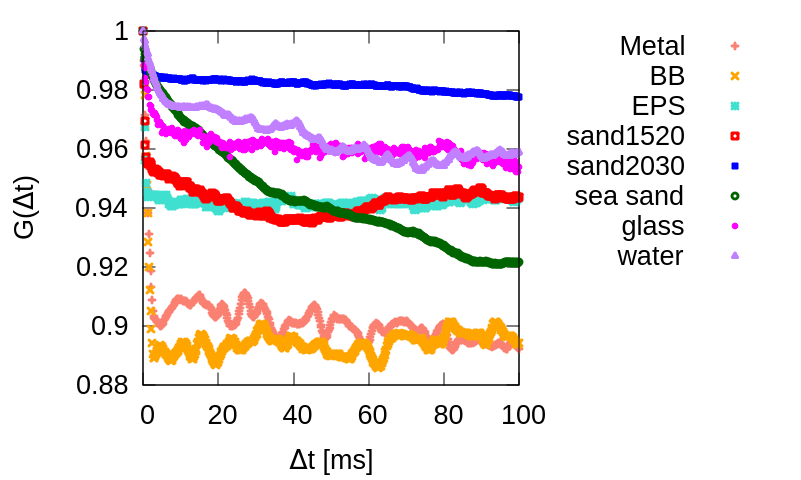
\includegraphics[scale=0.4]{multi.png}
	\caption{各物体の相関関数}
	\label{fig:overall}
\end{figure}
多くの場合において初期状態($G(0)=1$,完全一致)から急激な減少が起こっていることがわかる。$0 \leq \Delta t \leq 4 [ms]$を拡大したグラフが図\ref{fig:init}である。このグラフの結果から各粉粒体を3つのグループに分類した。第1グループは粒径6 mmを超えるものである。金属球(Metal)とBB弾(BB)がこれに当たる。グループ1は図\ref{fig:init}の範囲において2つの期間に分かれている。1つは$0 \leq \Dt \leq 2.5$にある相関が減少する区間である。これを区間Iと呼ぶ。もう1つはほぼ相関が一定になる区間\II である。2つの区間には明確な境界があり、2.5〜2.8 msと見られる。また区間\II については他のグループよりも振動が大きい。振動が大きい理由としては球が離散体として運動するため、確率的にベースフレームとほとんど一致しないフレームがあるからである。 \par
これよりも小さく粒径1 mm以上のものをグループ2とする。発泡ポリスチレン(EPS)と砂15-20メッシュ(sand1520)が含まれる。このグループについてもグループ1と同様2つの区間が見られるが、区間Iの時間がグループ1よりも短くなっている。境界は1 msあたりである。 \par
最後に残りをグループ3とする。これらは粒径が1 mmに満たない粒子径もしくは液体である。グループ3は特に海砂以下については区間Iが消失しているように見える。砂(20-30メッシュ)に関しては0.5 ms付近に境界があることが確認できるので、境界が見られない粉粒体については、より短い間隔で撮影を行うことで区間Iを発見することができると思われる。\par
区間Iと区間\II の境界を「相関持続時間$t_c$」とする。目視の範囲でわかる$t_c$を表\ref{tb:tc_eye}にまとめる。
\begin{figure}[H]
	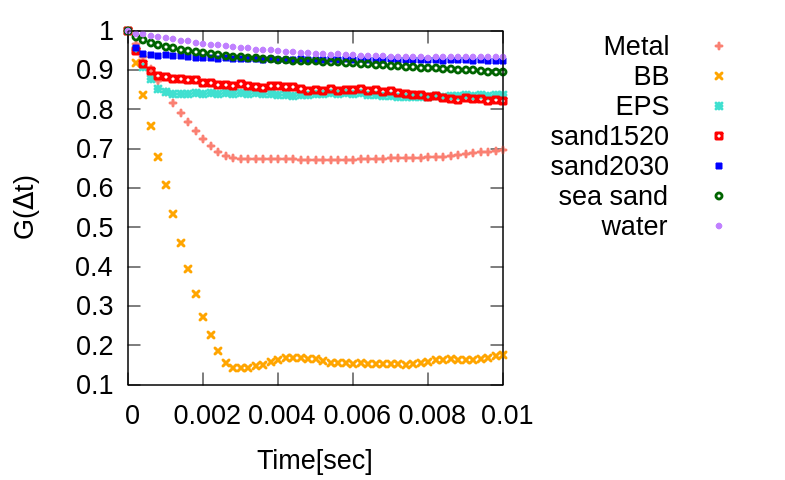
\includegraphics[scale=0.4]{init.png}
	\caption{各物体の相関関数(0.004秒まで)}
	\label{fig:init}
\end{figure}

\begin{table}[H]
	\caption{相関持続時間(目視) \label{tb:tc_eye}}
	\begin{tabular}{lr}
		\toprule
		グループ & $t_c [ms]$ \\
		\midrule
		グループ1 & 2.5-2.8 \\
		グループ2 & 1 \\
		グループ3(砂(20-30メッシュ)) & 0.5 \\
		グループ3(その他) & - \\
		\bottomrule
	\end{tabular}
\end{table}

\subsection{微分を用いた相関持続時間$t_c$の算出}
前述したように相関持続時間$t_c$は目視により大体の検討をつけることができるが、軸の縮尺等によって見え方は変わってくる。そこで、見た目という定性的な分析法ではなく、微分を用いて定量的に$t_c$を求めた。図\ref{fig:diff}は自己相関関数を時間差で微分したグラフである。 \par
自己相関関数は区間Iでは負の傾きを持つが、区間\II は0に近い傾きで振動する。そのため微分$\frac{dG(\Dt)}{\Dt}$で0付近になるときの時間差$\Dt がt_c$と一致すると考えられる。
\begin{figure}[H]
	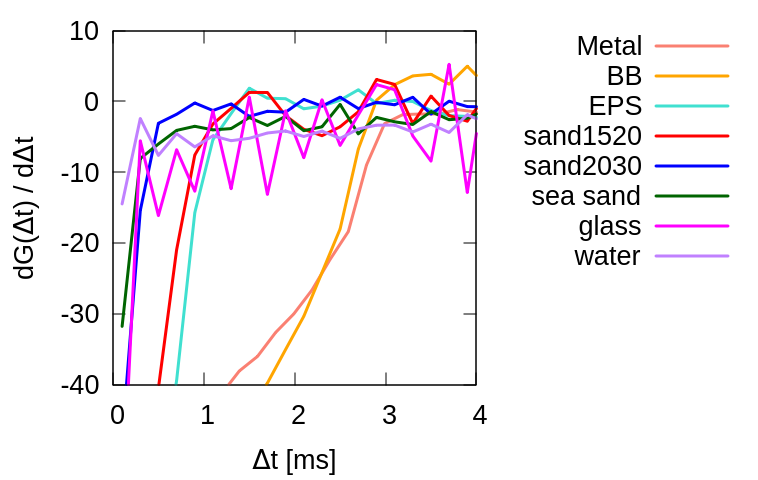
\includegraphics[scale=0.4]{diff.png}
	\caption{各物体の相関関数の微分}
	\label{fig:diff}
\end{figure}
微分を用いる場合、傾きが-10になるときの$\Dt$を調べることで目視とおおよそ一致することがわかった。表\ref{tb:tc_diff}に各グループの微分値が-10になるおおよその時間を示す。
\begin{table}[H]
	\caption{相関持続時間 \label{tb:tc_diff}}
	\begin{tabular}{lrr}
		\toprule
		%グループ & $t_c [ms](微分)$ & $t_c [ms](目視)$ \\
		グループ & $t_c [ms](微分)$  \\
		\midrule
		%グループ1 & 2.7 & 2.5-2.8 \\
		%グループ2 & 0.8 & 1 \\
		%グループ3(砂(20-30メッシュ)) & 0.4 & 0.5 \\
		%グループ3(その他) & 0.2 & - \\
		グループ1 & 2.7  \\
		グループ2 & 0.8  \\
		グループ3(砂(20-30メッシュ)) & 0.4  \\
		グループ3(その他) & 0.2 \\
		\bottomrule
	\end{tabular}
\end{table}

\subsection{グループ1の比較}
グループ1は相関減少区間(区間I)と一定になる区間(区間\II )が明確に分かれていることが特徴である。グループ1の自己相関関数を図\ref{fig:one}に示す。グループ1に属する金属球(Metal, 6.2 mm)とBB弾(BB, 6.0 mm )で大きな差はみられない。これは粒径のさがあまりないためであると考えられる。測定した粉粒体の種類が少ないので完全に傾向を予想することはできないが、自己相関関数の概形は粒径にのみに影響され、種類にはよらないものと思われる。
\begin{figure}[H]
	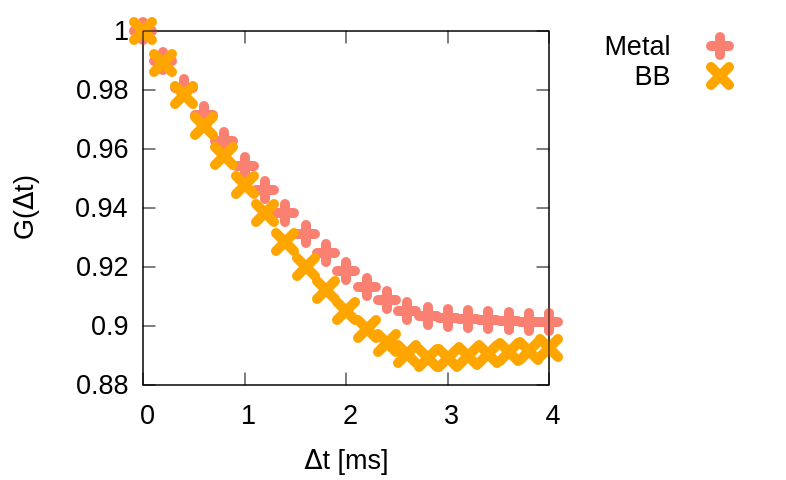
\includegraphics[scale=0.4]{one.png}
	\caption{グループ1の自己相関関数}
	\label{fig:one}
\end{figure}
\subsection{グループ2の比較}
グループ2の発泡ポリスチレンと砂(15-20メッシュ)は微分後の形を見ても明らかなように粒径が細かい砂の方が相関減少時間が短い。その結果砂のほうが区間\II 時点の値は大きい。このグループのように落下粉粒体を連続体として捉えることができる場合、相関減少は連続体の帯のヘリとその周辺の変化を表している。すなわち相関減少がより少ない砂は発泡ポリスチレンよりもヘリの変化が少ないということが言える。
\begin{figure}[H]
	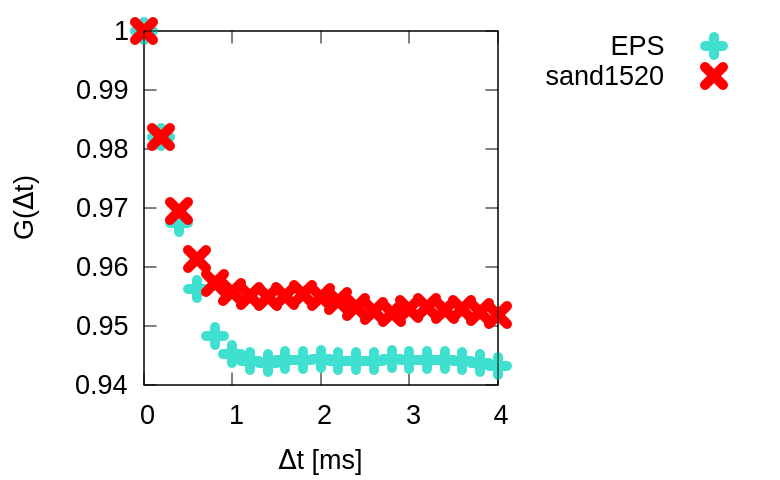
\includegraphics[scale=0.4]{two_big.png}
	\caption{グループ2の自己相関関数}
	\label{fig:two}
\end{figure}
\subsection{グループ3の比較}
グループ3の自己相関関数の形はそれぞれ個性的な形をしている。まず、砂(20-30メッシュ)はグループ1,2の傾向を引き継ぎ、相関減少時間を0.5 msと短くし、以降相関をほぼ一定に保っている。この区間分けができるのは砂(20-30メッシュ)までとなる。まず1つ細かい海砂には区間\II が見られず、解析限界の100 ms, G=0.92まで緩やかに減少を続けている。60 ms付近でグループ2の相関を追い抜いている。ただし減少速度は8つの中でも遅いため4 msという短い間隔で見れば典型的なグループ3として分類できる。ガラスビーズや水の相関には再び2つの区間が現れる。しかも5~6 msというグループ1よりも長い時間減少する。ガラスビーズと水についても海砂と同じく相関は0.95以上という高い値を保っている。
\begin{figure}[H]
	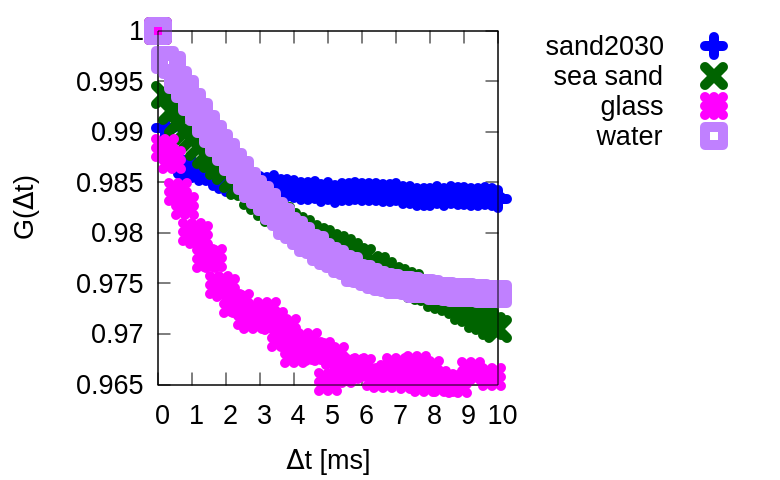
\includegraphics[scale=0.4]{three_up.png}
	\caption{グループ3の自己相関関数}
	\label{fig:three}
\end{figure}
\subsection{球(離散体)と粉(連続体)の相関減少の相違}
グループ3における相関減少時間と相関減少速度から海砂以下について次の予測が立てられる。粒径が小さくなると一旦相関減少時間は長くなるということである。そもそもグループ1に代表される離散体の相関減少区間は、初期位置からの球1つ分の移動を表していた。これはグループ2から少し意味が変わってくる。グループ2より粒径が細かくなると映像に帯、すなわち連続体の部分が現れるのである。連続体部分の相関減少はヘリの小さな変化に起因している。つまりグループ2の相関減少は離散体と連続体両方の要素を含んでいる。そしてグループ3には連続体のみが写っている。連続体の変化は離散体よりもずっと小さいため相関減少速度も小さくなる。そのためグループ1よりも減少時間が長くなるものと考えられる。ただし、減少が緩やかな分区間\II との区別がつきづらくなる。本研究では、減少後の相関値が高いため、全体的な傾向としてグループ3は相関減少時間が0.5 ms以下で曖昧または消失したものとしてまとめている。
\section{透過な物体の測定方法検討}
自己相関関数の計算には二値化画像処理が不可欠である。二値化する条件は被写体と背景の色のギャップが大きいことである。しかし、透明な物体は背景を透過するため二値化に十分なギャップを作ることができない。そこで、別な方法により二値化に似た処理を提案する。 \par
今回注目したのは透明な物体が背景を透過するとき、完全に背景を映し出さないという性質である。つまり透明な物体であっても多くの場合背景が歪んで見え、その物体を認識することができる。これを利用して背景の歪みを検出するプログラムを作成した。この測定法には背景に方眼紙(図\ref{fig:block})を用いる。
\begin{figure}[H]
	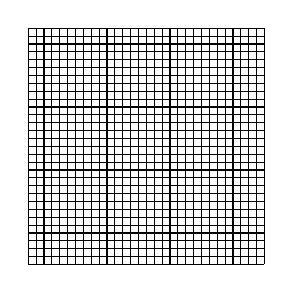
\begin{tikzpicture}
		\draw[step = 1 mm] (0,3) grid (3,0);
	\end{tikzpicture}
	\caption{背景(1 mm方眼)}
	\label{fig:block}
\end{figure}
図\ref{fig:block}を背景にし、透明な物体を落下運動させる。この映像を二値化し、線分を検出する。この段階では背景や光の反射によって物体の色が安定しない。だが、物体がない場所はそのまま線が映っているため線が検出できるが、物体がある場所は線が見えなくなるため検出できなくなる。次に真っ白で大きさが映像のものと同じ画像を用意する。これに線分を検出した場所に沿って太い線を引く。すると背景部分の多くが黒く塗りつぶされるため擬似的に透明物体を白く抜き出すことができる。図\ref{fig:line}に透明物体の落下画像(初期二値化済み)と疑似二値化画像を示す。
\begin{figure}[H]
	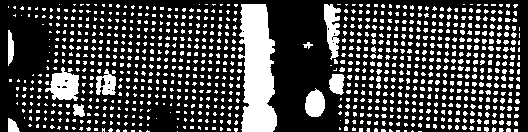
\includegraphics[scale=0.4]{water_two.png}
	
\includegraphics[scale=0.4]{water_line.png}
	\caption{落下映像(上)と疑似二値化画像(下)}
	\label{fig:line}
\end{figure}
\end{document}
